\documentclass[final,5p,times,twocolumn,authoryear]{elsarticle}
\usepackage[utf8]{inputenc}
\usepackage[T1]{fontenc}
\usepackage{graphicx}
\graphicspath{{./}{classification/}{eda/}{gradcam/}{pseudo_labeling_v2/}{segmentation_v1/}{segmentation_gtok/}{app_demo/}}
\usepackage{amsmath}
\usepackage[round,authoryear]{natbib}
\usepackage{url}
\usepackage{booktabs}
\usepackage{multirow}
\usepackage{xcolor}
\usepackage{tikz}
\usetikzlibrary{arrows.meta, positioning, fit, calc}
\usepackage{dblfloatfix}
\usepackage{adjustbox}
\usepackage{placeins}

\setcounter{topnumber}{5}
\setcounter{bottomnumber}{5}
\setcounter{totalnumber}{8}
\setcounter{dbltopnumber}{5}
\renewcommand{\topfraction}{0.95}
\renewcommand{\bottomfraction}{0.9}
\renewcommand{\textfraction}{0.05}
\renewcommand{\floatpagefraction}{0.85}
\renewcommand{\dbltopfraction}{0.95}
\renewcommand{\dblfloatpagefraction}{0.85}

\definecolor{stageblue}{HTML}{DCEBFF}
\definecolor{stagegreen}{HTML}{DDF4E7}
\definecolor{stageorange}{HTML}{FFE8CC}
\definecolor{stagegray}{HTML}{EEF1F5}
\definecolor{stagepurple}{HTML}{EDE4FF}
\definecolor{arrowgray}{HTML}{4B5563}

\tikzset{
    pipelinebox/.style={
        draw=arrowgray,
        rounded corners=2pt,
        align=center,
        minimum width=3.1cm,
        minimum height=1.15cm,
        font=\small,
        inner sep=5pt
    },
    data/.style={pipelinebox, fill=stagegray},
    classmodel/.style={pipelinebox, fill=stageblue},
    xai/.style={pipelinebox, fill=stageorange},
    sam/.style={pipelinebox, fill=stagepurple},
    segmodel/.style={pipelinebox, fill=stagegreen},
    flow/.style={-{Latex[length=2.6mm]}, thick, draw=arrowgray},
    dashedflow/.style={-{Latex[length=2.6mm]}, thick, dashed, draw=arrowgray},
    lane/.style={draw=arrowgray!45, rounded corners=4pt, inner sep=8pt}
}

\begin{document}

\begin{frontmatter}

\journal{Data and Information Management}

\title{An explainable weakly supervised framework for durian leaf disease classification and lesion segmentation using EfficientNet and U-Net}

\author[aff1]{Van Lam Ho}
\author[aff2]{Minh Hieu Doan\corref{cor1}}
% TODO: Replace with the corresponding author's institutional email before submission.
% \ead{corresponding.author@institution.edu}
\author[aff3]{Nguyen Quynh Nhi Tran}

\cortext[cor1]{Corresponding author.}

\affiliation[aff1]{
    organization={Faculty of Information Technology, Quy Nhon University},
    city={Gia Lai},
    country={Vietnam}
}

\affiliation[aff2]{
    organization={Quy Nhon AI Research and Application Center, FPT Software},
    city={Gia Lai},
    country={Vietnam}
}

\affiliation[aff3]{
    organization={Faculty of Mathematics and Computer Science, Dalat University},
    city={Lam Dong},
    country={Vietnam}
}

\begin{abstract}
Accurate detection of durian (\textit{Durio zibethinus}) leaf disease is important for orchard management, but pixel-level lesion annotation remains costly and depends on expert judgement. This study develops a weakly supervised workflow that starts from image-level disease labels and produces both class predictions and lesion masks. An EfficientNet-B0 classifier first learns five durian leaf classes and reaches 97.19\% test accuracy (weighted F1 97.19\%, macro ROC-AUC 99.87\%, $n=890$). Four weakly supervised segmentation experiments (E1--E4) are then trained from different pseudo-label sources -- raw Grad-CAM thresholding (E1), multi-scale GradCAM++ percentile masks (E2), SAM-refined masks under a dual-condition acceptance guard (E3), and GradCAM++ intersected with a disease-color prior (E4) -- and a post-processing fusion configuration (F1) that linearly combines the E2, E3, and E4 probability maps. Because pseudo-label-based test scores are circular (each experiment is flattered by evaluation against its own noisy label source), all localization claims are anchored to GT\_OK, an 80-image hand-labeled ground-truth set independent of any pseudo-label pipeline. On GT\_OK, the fusion configuration F1 reaches the best IoU (0.3083) and Dice (0.4713) of all evaluated configurations, tuned on 40 GT\_OK images and confirmed on the other 40 as a holdout (holdout IoU 0.3076, essentially unchanged from the full-80 figure). No single checkpoint exceeds IoU~0.22 on GT\_OK, and F1's precision (0.41) remains modest, so the result is best read as the strongest available configuration under a disclosed, controlled recipe rather than a solved segmentation problem. We further show that SAM's dual-condition guard (IoU~$\geq$~0.15 and a 0.35--2.0$\times$ coverage-ratio bound) still under-constrains mask expansion, since observed class-wise expansion ratios reach 1.4--2.0$\times$, at the edge of the guard's own tolerance. A Streamlit demonstration application exposes the full pipeline -- classification, GradCAM overlay, and a selectable E1--E4 segmentation checkpoint -- for interactive inspection. These results support the use of classifier explanations as a practical source of weak spatial supervision, while showing precisely where such supervision, and its evaluation, need careful checking.
\end{abstract}

\begin{keyword}
Durian leaf disease \sep Deep learning \sep EfficientNet \sep GradCAM++ \sep Pseudo-labeling \sep UNet++ \sep Segment Anything Model \sep Weakly supervised segmentation \sep Model fusion \sep Agricultural AI
\end{keyword}

\end{frontmatter}

\section{Introduction}

Durian (\textit{Durio zibethinus}) is one of the most economically significant tropical fruit crops in Southeast Asia, with Thailand, Malaysia, Indonesia, and Vietnam among the leading producers. Because fruit quality and yield are highly sensitive to foliar health, leaf diseases represent a persistent threat to grower income and to the sustainability of durian cultivation. Timely and accurate identification of disease symptoms is needed for targeted intervention, judicious use of agrochemicals, and crop management at plantation scale.

Conventional disease diagnosis relies on visual inspection by trained agronomists. This practice is labour-intensive, subjective, and difficult to scale to large orchards, and it typically identifies a problem only after symptoms have become severe. The maturation of deep learning and computer vision has motivated a large body of work on automated plant disease recognition, which now routinely achieves high classification accuracy across many crops \citep{mohanty2016using, ferentinos2018deep}. However, two gaps limit the practical value of most existing systems for durian. First, the majority of methods perform image-level classification only: they report \emph{whether} a leaf is diseased but not \emph{where} the lesions are, whereas spatial localization is what enables precise, site-specific treatment. Second, models that do produce pixel-level segmentation depend on dense manual annotation, which is costly, slow, and requires domain expertise that is rarely available for a specialty crop such as durian.

This work addresses three coupled challenges in durian leaf disease analysis:
\begin{enumerate}
\item \textbf{Annotation scarcity.} Pixel-level masks for plant lesions are expensive and expert-dependent; most accessible durian data carry only image-level labels.
\item \textbf{Interpretability.} Opaque deep models are difficult for agronomists to trust or validate, which impedes adoption in the field.
\item \textbf{Precise localization.} Classification alone cannot delineate the position and extent of lesions, information that is essential for targeted, resource-efficient treatment.
\end{enumerate}

To address these issues, we use an image-level classifier as the starting point for lesion segmentation. Class activation maps provide the initial spatial cues, SAM is used as a boundary refinement step under an explicit acceptance guard, and a small hand-labeled evaluation set (GT\_OK) is introduced so that localization quality can be judged independently of the pseudo-labels used for training. The main contributions are:
\begin{itemize}
\item A weakly supervised workflow linking classification, GradCAM/GradCAM++ pseudo-labeling, SAM refinement, a disease-color prior, and UNet++ segmentation using only image-level labels, instantiated as four segmentation experiments (E1--E4) that isolate the effect of the pseudo-label source.
\item A post-processing fusion configuration (F1) that linearly combines three checkpoints' probability maps under a per-class threshold and coverage cap, tuned and held out on disjoint halves of an 80-image ground-truth set.
\item GT\_OK, an 80-image hand-labeled evaluation set used as the sole basis for localization claims, together with an explicit contrast against the circular ``pseudo-test'' metric (evaluating a checkpoint against labels of the same kind used to train it) that earlier pseudo-label-only evaluation protocols relied on.
\item An analysis of SAM ViT-B as a label refiner under a dual-condition guard (a minimum IoU together with a bounded coverage ratio), showing that the guard's own upper bound is still looser than the mask-expansion ratios observed in practice.
\item A working Streamlit demonstration application exposing classification, GradCAM explanation, and a selectable E1--E4 segmentation checkpoint for interactive use.
\end{itemize}

The remainder of the paper is organised as follows. Section~\ref{sec:related} reviews related work on plant disease detection, explainable AI, weakly supervised segmentation, and segmentation foundation models. Section~\ref{sec:method} describes the dataset and the stages of the method, including the four segmentation experiments, the fusion configuration, and the GT\_OK evaluation set. Section~\ref{sec:results} reports and discusses the experimental results, including the pseudo-test versus GT\_OK evaluation-design caveat and the SAM expansion analysis. Section~\ref{sec:conclusion} concludes and outlines future directions.

\section{Related work}
\label{sec:related}

\subsection{Deep learning for plant disease detection}

Convolutional neural networks (CNNs) have become the standard tool for image-based plant disease recognition, with successful applications across crops such as tomato, rice, and wheat \citep{mohanty2016using, ferentinos2018deep}. Because agricultural datasets are typically small relative to general-purpose vision corpora, transfer learning from ImageNet-pretrained backbones such as VGG, ResNet, and EfficientNet is common practice \citep{deng2009imagenet, tan2019efficientnet}. EfficientNet in particular offers a favourable accuracy-to-parameter trade-off through compound scaling of network depth, width, and input resolution \citep{tan2019efficientnet}, which makes it attractive for deployment-constrained agricultural settings. Most of these systems, however, stop at image-level classification and cannot indicate the spatial location or extent of the disease, limiting their usefulness for targeted treatment.

\subsection{Explainable AI in agricultural vision}

Interpretability matters in agricultural decision support because users need to know whether a model is responding to disease symptoms or to background cues. Gradient-weighted Class Activation Mapping (Grad-CAM) and related methods show which image regions influence a prediction \citep{selvaraju2017grad}. GradCAM++ improves localization for multiple and small objects by using second-order gradient information \citep{chattopadhay2018grad}, which is relevant for leaf diseases that often appear as scattered lesions. In this study, class activation maps are used not only for inspection but also as weak spatial supervision for segmentation, and are exposed directly to end users through the demonstration application described in Section~\ref{sec:demo}.

\subsection{Weakly supervised segmentation and pseudo-labeling}

Weakly supervised segmentation aims to estimate pixel-level masks from cheaper labels such as image tags. Class activation maps are often used for this purpose because they provide coarse localization cues that can be thresholded and post-processed into pseudo-masks \citep{barbedo2019plant}. The main difficulty is that CAMs are low-resolution and often cover only the most discriminative part of an object. Pseudo-label quality depends heavily on thresholding and post-processing, and, critically, on how the resulting models are evaluated: a model scored against pseudo-labels of the same kind used to train it will appear far stronger than it is against independent ground truth, an evaluation-design pitfall we quantify directly in Section~\ref{sec:pseudotest}. In Section~\ref{sec:stage2v2}, we use multi-scale fusion together with per-class percentile thresholds as a practical alternative to Otsu thresholding, whose bimodality assumption is poorly matched to smooth fused heatmaps \citep{otsu1979threshold}.

\subsection{Segmentation foundation models}

The Segment Anything Model (SAM) is a promptable segmentation model trained on eleven million images and over one billion masks \citep{kirillov2023segment}. Given point, box, or mask prompts, SAM can produce sharp object boundaries and has been used in settings where manual annotation is limited. Here, SAM is not treated as a stand-alone disease segmenter. It is used as a refinement step for coarse GradCAM++ pseudo-masks, and its behaviour is checked for both boundary improvement and mask expansion under an explicit dual-condition guard (Section~\ref{sec:samguard}). The segmentation networks used in the experiments build on U-Net \citep{ronneberger2015unet} and the nested UNet++ variant \citep{zhou2018unet++}.

\subsection{Positioning of this work}

Compared with previous work, this study focuses on a durian-specific setting with image-level labels only. It combines GradCAM++ pseudo-labeling, SAM refinement, and a disease-color prior across four segmentation experiments (E1--E4), fuses the strongest three under a disclosed post-processing recipe (F1), and evaluates every configuration against an independent hand-labeled set (GT\_OK) rather than against each experiment's own pseudo-labels. This distinction is important because pseudo-label-based scores can be misleading when each model is evaluated against labels produced by a different, and possibly self-serving, procedure.

\section{Materials and methods}
\label{sec:method}

\begin{figure*}[!t]
\centering
\resizebox{\textwidth}{!}{%
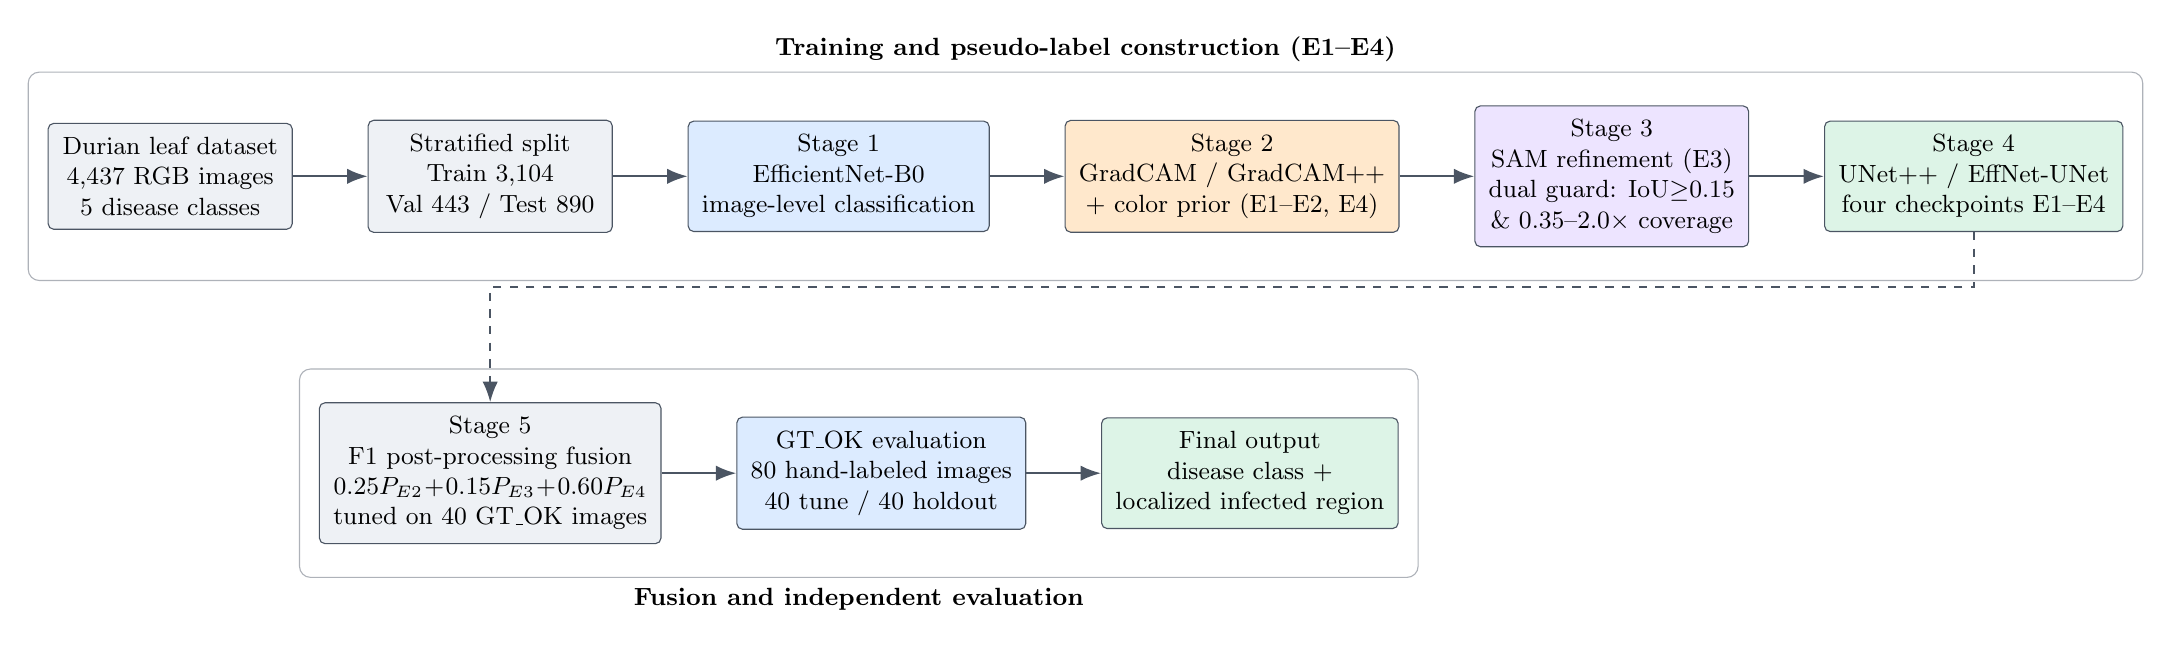
\begin{tikzpicture}[node distance=0.85cm and 0.95cm]
    \node[data] (dataset) {Durian leaf dataset\\4,437 RGB images\\5 disease classes};
    \node[data, right=of dataset] (split) {Stratified split\\Train 3,104\\Val 443 / Test 890};
    \node[classmodel, right=of split] (classifier) {Stage 1\\EfficientNet-B0\\image-level classification};
    \node[xai, right=of classifier] (gradcam) {Stage 2\\GradCAM / GradCAM++\\+ color prior (E1--E2, E4)};
    \node[sam, right=of gradcam] (samrefine) {Stage 3\\SAM refinement (E3)\\dual guard: IoU$\geq$0.15\\\& 0.35--2.0$\times$ coverage};
    \node[segmodel, right=of samrefine] (segtrain) {Stage 4\\UNet++ / EffNet-UNet\\four checkpoints E1--E4};

    \node[data, below=2.15cm of split] (fusion) {Stage 5\\F1 post-processing fusion\\$0.25P_{E2}\!+\!0.15P_{E3}\!+\!0.60P_{E4}$\\tuned on 40 GT\_OK images};
    \node[classmodel, right=of fusion] (gtok) {GT\_OK evaluation\\80 hand-labeled images\\40 tune / 40 holdout};
    \node[segmodel, right=of gtok] (decision) {Final output\\disease class +\\localized infected region};

    \draw[flow] (dataset) -- (split);
    \draw[flow] (split) -- (classifier);
    \draw[flow] (classifier) -- (gradcam);
    \draw[flow] (gradcam) -- (samrefine);
    \draw[flow] (samrefine) -- (segtrain);

    \draw[dashedflow] (segtrain.south) -- ++(0,-0.7) -| (fusion.north);
    \draw[flow] (fusion) -- (gtok);
    \draw[flow] (gtok) -- (decision);

    \node[lane, fit=(dataset)(split)(classifier)(gradcam)(samrefine)(segtrain), inner xsep=7pt, inner ysep=12pt,
        label={[font=\bfseries\small]above:Training and pseudo-label construction (E1--E4)}] {};
    \node[lane, fit=(fusion)(gtok)(decision), inner xsep=7pt, inner ysep=12pt,
        label={[font=\bfseries\small]below:Fusion and independent evaluation}] {};
\end{tikzpicture}%
}
\caption{Overview of the proposed weakly supervised durian leaf disease analysis workflow. The classification model learns image-level disease categories; four pseudo-label sources (raw Grad-CAM, GradCAM++ percentile masks, SAM-refined masks, and GradCAM++ intersected with a disease-color prior) each train a segmentation checkpoint (E1--E4). A post-processing fusion (F1) linearly combines the E2, E3, and E4 probability maps, and every configuration is scored against GT\_OK, an 80-image hand-labeled evaluation set held independent of the pseudo-label pipeline.}
\label{fig:proposed_pipeline}
\end{figure*}

\subsection{Dataset}

The dataset comprises 4{,}437 durian leaf images collected from plantations in Southeast Asia, organised into five classes: Algal Leaf Spot (733 images), Allocaridara Attack (913 images), Healthy Leaf (976 images), Leaf Blight (937 images), and Phomopsis Leaf Spot (878 images).

\begin{figure*}[!t]
\centering
\includegraphics[width=\textwidth]{eda/sample_images_per_class.png}
\caption{Representative samples from the five durian leaf classes used in the experiments, illustrating the visual diversity of healthy leaves and disease symptoms under field imaging conditions.}
\label{fig:dataset_samples}
\end{figure*}

The data were partitioned into training (70\%, 3{,}104 images), validation (10\%, 443 images), and test (20\%, 890 images) sets by stratified sampling to preserve the class distribution. For the segmentation stages, the same 3{,}104 training images were used for pseudo-label generation across all four experiments (E1--E4), with a fixed seed (42) to ensure reproducibility and a consistent comparison basis.

\subsection{Stage 1: Image-level classification}

\subsubsection{Architecture}

We adopt EfficientNet-B0 as the classification backbone for its favourable balance between accuracy and computational cost \citep{tan2019efficientnet}. The network takes $224\times224\times3$ RGB inputs, applies an ImageNet-pretrained EfficientNet-B0 backbone \citep{deng2009imagenet}, global average pooling, a fully connected layer with five outputs, and a softmax activation.

\subsubsection{Training configuration}

The classifier was optimised with Adam (learning rate $1\times10^{-4}$) under a cross-entropy objective, a batch size of 32, and up to 30 epochs with learning-rate reduction on plateau (ReduceLROnPlateau, patience~=~2, factor~=~0.5). Data augmentation comprised random horizontal and vertical flips, rotation, and colour jitter.

\subsubsection{Results}

The model reached 97.19\% test accuracy with a mean confidence of 0.9803 on correctly classified test images. Consistently high-confidence predictions are important because they yield reliable class activation maps to serve as segmentation seeds for the pseudo-label pipeline.

\subsection{Segmentation experiments overview}
\label{sec:seg_overview}

Rather than a single segmentation checkpoint, we train four segmentation experiments that isolate the effect of the pseudo-label source while holding the surrounding training recipe fixed, plus one post-processing fusion configuration (Table~\ref{tab:exp_overview}). E1 reproduces a simple, low-cost baseline; E2 and E4 test two different ways of sharpening the classifier's spatial signal (multi-scale GradCAM++ and a disease-color prior, respectively); E3 tests whether SAM's boundary refinement helps once it is accepted only under a dual-condition guard; and F1 tests whether combining checkpoints in a controlled, disclosed way is preferable to picking any single one.

\begin{table}[!htbp]
\centering
\caption{Segmentation experiments: pseudo-label source, model, and role.}
\label{tab:exp_overview}
\begin{adjustbox}{max width=\columnwidth}
\begin{tabular}{lllp{3.1cm}}
\toprule
\textbf{Exp.} & \textbf{Pseudo-label source} & \textbf{Model} & \textbf{Role} \\
\midrule
E1 & Raw Grad-CAM threshold masks & EfficientNet-U-Net (custom decoder) & Baseline \\
E2 & GradCAM++ percentile masks & UNet++ (EfficientNet-B0 encoder) & Improves heatmap quality over E1 \\
E3 & SAM-refined V2 masks, coverage guard & UNet++ (EfficientNet-B0 encoder) & Tests whether SAM boundary refinement helps \\
E4 & GradCAM++ $\cap$ disease-color prior & UNet++ (EfficientNet-B0 encoder) & Best single checkpoint on GT\_OK \\
\midrule
F1 & Post-processing fusion of E2, E3, E4 & --- (no separate training) & Best overall configuration on GT\_OK \\
\bottomrule
\end{tabular}
\end{adjustbox}
\end{table}

\subsection{Stage 2 (E1, baseline): single-scale GradCAM pseudo-labels}

As a baseline, single-layer Grad-CAM was applied to the final convolutional layer (\texttt{features.8}, $7\times7$ resolution) with a fixed threshold of 0.5 and a rectangular $5\times5$ morphological kernel, on a 500-image subset (100 per class). This configuration defines the segmentation baseline referred to as E1 in Section~\ref{sec:seg_results}.

\subsection{Stage 2 (E2): multi-scale GradCAM++ with per-class percentile thresholding}
\label{sec:stage2v2}

\subsubsection{Multi-scale GradCAM++}

Single-scale Grad-CAM often fails to capture multiple small lesions because of spatial averaging. We combine GradCAM++ activations from two resolution levels. Fine-grained features ($14\times14$, \texttt{features.6}) improve the localization of small lesions and preserve spot detail, whereas coarse features ($7\times7$, \texttt{features.8}) provide semantic context and suppress background false positives. The fused heatmap is
\begin{equation}
H_{final} = 0.6 \times H_{fine} + 0.4 \times H_{coarse}.
\end{equation}
GradCAM++ refines standard Grad-CAM by weighting activations with second-order gradient information \citep{chattopadhay2018grad}:
\begin{equation}
\alpha_k^c = \frac{\frac{\partial^2 y^c}{\partial A_k^2}}{2\frac{\partial^2 y^c}{\partial A_k^2} + \sum A_k \frac{\partial^3 y^c}{\partial A_k^3}},
\end{equation}
\begin{equation}
w_k^c = \sum \alpha_k^c \times \text{ReLU}\left(\frac{\partial y^c}{\partial A_k}\right),
\end{equation}
where $A_k$ denotes activation maps and $y^c$ the class score.

\subsubsection{Per-class percentile thresholding}

Rather than Otsu's method \citep{otsu1979threshold}, which assumes a bimodal heatmap distribution and over-segments when multi-scale fusion produces smooth gradients, we apply a per-class percentile threshold that directly controls mask coverage (Table~\ref{tab:percentile}).

\begin{table}[!htbp]
\centering
\caption{Per-class coverage targets for percentile thresholding.}
\label{tab:percentile}
\begin{adjustbox}{max width=\columnwidth}
\begin{tabular}{lcc}
\toprule
\textbf{Class} & \textbf{Keep top \%} & \textbf{Rationale} \\
\midrule
Algal Leaf Spot     & 18\% & Compact spot lesions \\
Allocaridara Attack & 20\% & Moderate-area insect damage \\
Healthy Leaf        & 0\%  & No lesion tissue \\
Leaf Blight         & 22\% & Diffuse blight patches \\
Phomopsis Leaf Spot & 18\% & Compact spot lesions \\
\bottomrule
\end{tabular}
\end{adjustbox}
\end{table}

The threshold is the $(1-p)\times100^{\text{th}}$ percentile of each heatmap, where $p$ is the target coverage fraction. Assigning Healthy Leaf an all-zero mask removes the $\sim$683 false-positive masks that would otherwise be generated for disease-free images. The trade-off is that coverage is fixed per class and does not adapt to disease severity in each image.

\subsubsection{Post-processing}

Two post-processing steps clean the thresholded masks: (i) morphological closing followed by opening with a $5\times5$ elliptical kernel to fill holes and remove noise, and (ii) connected-component filtering that retains the top three components of at least 400 pixels, removing mid-size noise fragments while preserving multiple lesion spots. This procedure produced 3{,}104 pseudo-labeled masks from the full training set and defines the E2 pseudo-label source.

\begin{figure*}[!t]
\centering
\includegraphics[width=\textwidth]{gradcam/gradcam_samples_per_class_landscape.png}
\caption{GradCAM++ activation maps for representative samples from each disease class. The heatmaps mark the regions used by the classifier and are later thresholded to generate pseudo-segmentation masks.}
\label{fig:gradcam_samples}
\end{figure*}

\begin{figure*}[!t]
\centering
\includegraphics[width=\textwidth]{pseudo_labeling_v2/v1_vs_v2_comparison.png}
\caption{Pseudo-label quality: single-scale Grad-CAM (E1 source, fixed threshold 0.5) versus multi-scale GradCAM++ with per-class percentile thresholding (E2 source). The E2 approach produces coverage-controlled, cleaner masks, with noise fragments removed by top-3 connected-component filtering.}
\label{fig:pseudolabel_comparison}
\end{figure*}

\subsection{Stage 2 (E4): GradCAM++ intersected with a disease-color prior}
\label{sec:stage2v5}

E4 tests whether a simple, model-independent visual prior can compensate for the coverage errors of GradCAM++ alone. For each disease class, an empirical color prior (a set of hue/saturation ranges characteristic of the lesion appearance for that class, e.g. brown/necrotic tones for blight and pale chlorotic tones for algal spot) is computed over the training images and intersected pixel-wise with the E2 GradCAM++ percentile mask: a pixel is kept only if it is both activation-salient \emph{and} color-consistent with the disease class. This intersection removes GradCAM++ activation that falls on healthy leaf tissue or background, at the cost of also removing genuine lesion pixels whose color deviates from the class-typical range. The resulting masks train a UNet++ checkpoint with the same architecture and training recipe as E2/E3 (Section~\ref{sec:seg_train}). On GT\_OK (Section~\ref{sec:gtok}), E4 is the strongest single checkpoint, narrowly ahead of the E1 baseline and clearly ahead of E2 and E3, with recall (0.7455) substantially higher than its precision (0.2358), the same over-segmentation pattern observed across all four experiments.

\subsection{Stage 3: SAM boundary refinement (E3)}
\label{sec:samguard}

\subsubsection{Motivation and prompt generation}

GradCAM++ localises lesions well but yields blurry boundaries because of the low resolution of the activation maps ($7\times7$ or $14\times14$). SAM excels at pixel-accurate boundary delineation given suitable prompts \citep{kirillov2023segment}. For each E2 pseudo-mask we extract foreground prompts (the mask centroid plus five points sampled from the masked region) and background prompts (three points sampled from the dilated complement, using a 30-pixel dilation) so that SAM can distinguish diseased from healthy tissue.

\subsubsection{Dual-condition acceptance guard}

An earlier version of this pipeline accepted a SAM-refined mask whenever its IoU against the source GradCAM++ mask exceeded 0.15, with no other constraint. This one-sided rule has a specific failure mode: when SAM segments a much larger region that fully contains the source mask, the IoU reduces to (source coverage)/(SAM coverage), which can still clear the 0.15 threshold even though the refined mask has expanded far beyond the lesion. The pipeline used for E3 therefore applies a \emph{dual-condition} guard, requiring both a minimum IoU against the source mask and a bounded coverage (area) ratio between the SAM mask and the source mask:
\begin{equation}
\text{IoU} = \frac{|\text{SAM}_{mask} \cap \text{GradCAM}_{mask}|}{|\text{SAM}_{mask} \cup \text{GradCAM}_{mask}|},
\end{equation}
\begin{equation}
r = \frac{|\text{SAM}_{mask}|}{|\text{GradCAM}_{mask}|},
\end{equation}
\begingroup\footnotesize
\begin{equation}
\text{refined}_{mask} = \begin{cases}
\text{SAM}_{mask} & \text{IoU}\geq0.15,\ r\in[0.35,2.0], \\
\text{GradCAM}_{mask} & \text{otherwise.}
\end{cases}
\end{equation}
\endgroup
The lower bound on $r$ rejects SAM masks that shrink implausibly relative to the source; the upper bound is intended to reject the whole-leaf over-expansion described above.

\subsubsection{A known limitation of the guard's coverage bound}

The 2.0$\times$ upper bound on the coverage ratio was set as a conservative cap, but it is still looser than the class-wise mask-expansion ratios observed once SAM refinement is applied at scale (Table~\ref{tab:sam_expansion}): the ratio of SAM-refined coverage to E2 source coverage falls in roughly 1.4--2.0$\times$ across classes, i.e. at or just inside the guard's own tolerance. As a result, the guard reduces but does not eliminate over-expansion, and E3's GT\_OK precision (0.1409) is the lowest of the four experiments even though its recall (0.7685) is the highest -- SAM catches most of the true lesion but at the cost of a large false-positive area around it. We treat this as an explicit, disclosed limitation (Section~\ref{sec:limitations}) rather than tuning the bound post hoc to a value that happens to look better on this dataset.

\begin{table}[!htbp]
\centering
\caption{Coverage expansion from E2 pseudo-labels to SAM-refined (E3) labels.}
\label{tab:sam_expansion}
\begin{adjustbox}{max width=\columnwidth}
\begin{tabular}{lccc}
\toprule
\textbf{Class} & \textbf{E2 coverage} & \textbf{SAM coverage} & \textbf{Ratio $r$} \\
\midrule
Algal Leaf Spot     & 17.7\% & 35.0\% & 1.97$\times$ \\
Allocaridara Attack & 19.7\% & 32.0\% & 1.62$\times$ \\
Leaf Blight         & 21.7\% & 30.7\% & 1.41$\times$ \\
Phomopsis Leaf Spot & 17.6\% & 33.6\% & 1.91$\times$ \\
\bottomrule
\end{tabular}
\end{adjustbox}
\end{table}

\subsection{Stage 4: Lesion segmentation}
\label{sec:seg_train}

\subsubsection{Architecture}

E1 uses a custom EfficientNet-U-Net trained with a combined BCE and Dice loss (Adam with ReduceLROnPlateau, 30 epochs). E2, E3, and E4 use UNet++ \citep{zhou2018unet++} with an ImageNet-pretrained EfficientNet-B0 encoder, nested dense skip connections in the decoder, and a single-channel binary output (disease versus background); the model has 6{,}569{,}581 trainable parameters. The dense skip connections of UNet++ reduce the semantic gap between encoder and decoder and improve small-object segmentation relative to plain U-Net \citep{ronneberger2015unet}.

\subsubsection{Training configuration (E2--E4)}

The segmentation objective is a FocalDice loss:
\begin{equation}
\mathcal{L}_{total} = \mathcal{L}_{focal} + \mathcal{L}_{dice},
\end{equation}
\begin{equation}
\mathcal{L}_{focal} = -\alpha(1-p_t)^\gamma \log(p_t), \quad \alpha=0.25,\ \gamma=2.0,
\end{equation}
\begin{equation}
\mathcal{L}_{dice} = 1 - \frac{2|X \cap Y| + \epsilon}{|X| + |Y| + \epsilon},
\end{equation}
where the focal term follows \citet{lin2017focal}. Optimisation used AdamW \citep{loshchilov2019decoupled} (learning rate $1\times10^{-4}$, weight decay $1\times10^{-4}$), a CosineAnnealingLR schedule ($T_{max}=50$, $\eta_{min}=1\times10^{-6}$), a batch size of 4, up to 50 epochs with early stopping on validation loss (patience~=~10), and gradient clipping at a maximum norm of 1.0. Augmentation comprised RandomResizedCrop, horizontal/vertical flips, RandomRotate90, ShiftScaleRotate, ElasticTransform, GridDistortion, ColorJitter, and GaussNoise \citep{buslaev2020albumentations}. E1, E2, E3, and E4 share this recipe except for the architecture difference noted above and the pseudo-label source described in each experiment's subsection.

\subsection{Stage 5: F1 post-processing fusion}
\label{sec:fusion}

F1 is not a separately trained model; it is a fixed post-processing rule applied to the probability maps already produced by E2, E3, and E4 at inference time:
\begin{equation}
P_{F1} = 0.25\,P_{E2} + 0.15\,P_{E3} + 0.60\,P_{E4},
\end{equation}
followed by a per-class probability threshold and a per-class coverage cap. The weights favour E4 (the strongest single checkpoint) while still drawing on E2's higher precision and E3's higher recall. The threshold and coverage cap for each class were tuned by grid search on 40 of the 80 GT\_OK images (Section~\ref{sec:gtok}) to maximise IoU, and the resulting configuration was then evaluated, unchanged, on the other 40 GT\_OK images as a holdout set. E1 is intentionally excluded from the fusion weights: it uses a different architecture (EfficientNet-U-Net rather than UNet++) and a different pseudo-label distribution, and including it would mix probability maps that are not directly comparable in scale.

\subsection{GT\_OK: an independent ground-truth evaluation set}
\label{sec:gtok}

All of the segmentation experiments above are trained without any pixel-level ground truth. To judge localization quality without relying on the same noisy signal that generated the training labels, we hand-labeled 80 test images with pixel-accurate lesion masks (GT\_OK), independent of any pseudo-label pipeline. GT\_OK is split into 40 images used to tune F1's per-class threshold and coverage cap (Section~\ref{sec:fusion}) and 40 held out purely for evaluation. Every number reported as a segmentation result in Section~\ref{sec:results} unless explicitly marked otherwise is a GT\_OK score; this is a deliberate departure from evaluation protocols in earlier iterations of this pipeline that reported only pseudo-label-based test metrics, which are shown in Section~\ref{sec:pseudotest} to overstate localization quality considerably.

\subsection{Demonstration application}
\label{sec:demo}

To make the pipeline usable outside a notebook environment, we built a Streamlit web application that accepts an uploaded leaf image and runs the full pipeline live: EfficientNet-B0 classification, a GradCAM overlay, and a selectable UNet++ segmentation checkpoint (E1--E4, labeled by pseudo-label source as Baseline / GradCAM++ / SAM-refined / Color prior). The application exposes an inference-mode selector (model-only, model with color-prior post-processing, or a GradCAM~$\cap$~color-prior preview), a threshold slider (0.1--0.9), and a rule-based advisory panel that summarises disease severity from the predicted mask coverage, with an optional large-language-model-backed advisory mode. The application was re-verified running end to end on 2026-08-30.

\section{Results and discussion}
\label{sec:results}

\subsection{Classification performance}

EfficientNet-B0 achieved high test performance across all five classes (Table~\ref{tab:classification}), with similar per-class scores (Table~\ref{tab:classification_perclass}) and a macro ROC-AUC of 99.87\%.

\begin{table}[!htbp]
\centering
\caption{Classification performance on the test set ($n=890$).}
\label{tab:classification}
\begin{adjustbox}{max width=\columnwidth}
\begin{tabular}{lc}
\toprule
\textbf{Metric} & \textbf{Test} \\
\midrule
Accuracy          & 97.19\% \\
Weighted precision & 97.22\% \\
Weighted recall    & 97.19\% \\
Weighted F1        & 97.19\% \\
Macro ROC-AUC      & 99.87\% \\
\bottomrule
\end{tabular}
\end{adjustbox}
\end{table}

\begin{table}[!htbp]
\centering
\caption{Per-class classification performance on the test set.}
\label{tab:classification_perclass}
\begin{adjustbox}{max width=\columnwidth}
\begin{tabular}{lcccc}
\toprule
\textbf{Class} & \textbf{Precision} & \textbf{Recall} & \textbf{F1} & \textbf{Samples} \\
\midrule
Algal Leaf Spot     & 94.67\% & 96.60\% & 95.62\% & 147 \\
Allocaridara Attack & 95.74\% & 98.36\% & 97.04\% & 183 \\
Healthy Leaf        & 97.99\% & 99.49\% & 98.73\% & 196 \\
Leaf Blight         & 100.00\% & 96.81\% & 98.38\% & 188 \\
Phomopsis Leaf Spot & 97.08\% & 94.32\% & 95.68\% & 176 \\
\midrule
\textbf{Weighted avg.} & \textbf{97.22\%} & \textbf{97.19\%} & \textbf{97.19\%} & \textbf{890} \\
\bottomrule
\end{tabular}
\end{adjustbox}
\end{table}

\begin{figure*}[!t]
\centering
\includegraphics[width=\textwidth]{classification/training_curves.png}
\caption{Training and validation curves for the EfficientNet-B0 classifier. A test accuracy of 97.19\% is achieved with balanced per-class F1 scores of 0.96--0.99.}
\label{fig:classification_training_curves}
\end{figure*}

\begin{figure}[!htbp]
\centering
\includegraphics[width=\columnwidth]{classification/confusion_matrix.png}
\caption{Confusion matrix on the test set. Most misclassifications occur between visually similar classes, particularly Algal Leaf Spot and Phomopsis Leaf Spot.}
\label{fig:confusion_matrix}
\end{figure}

\subsection{Pseudo-label quality (E2 source)}

The E2 coverage targets were met with less than 0.4\% deviation per class (Table~\ref{tab:v2_coverage}). Setting Healthy Leaf coverage to zero removes the $\sim$683 false-positive masks that would otherwise arise for a disease-free class.

\begin{table}[!htbp]
\centering
\caption{E2 (GradCAM++ percentile) pseudo-label coverage statistics.}
\label{tab:v2_coverage}
\begin{adjustbox}{max width=\columnwidth}
\begin{tabular}{lccc}
\toprule
\textbf{Class} & \textbf{Actual coverage} & \textbf{Std} & \textbf{Target} \\
\midrule
Algal Leaf Spot     & 17.7\% & 0.008 & 18\% \\
Allocaridara Attack & 19.7\% & 0.007 & 20\% \\
Healthy Leaf        & 0.0\%  & 0.000 & 0\%  \\
Leaf Blight         & 21.7\% & 0.007 & 22\% \\
Phomopsis Leaf Spot & 17.6\% & 0.009 & 18\% \\
\bottomrule
\end{tabular}
\end{adjustbox}
\end{table}

\subsection{Segmentation performance on GT\_OK}
\label{sec:seg_results}

Table~\ref{tab:segmentation} reports every configuration's performance on GT\_OK, the 80-image hand-labeled evaluation set (Section~\ref{sec:gtok}), which we treat as the only trustworthy basis for localization claims in this study.

\begin{table}[!htbp]
\centering
\caption{Segmentation performance on GT\_OK (80 hand-labeled images; F1: 40-image holdout).}
\label{tab:segmentation}
\footnotesize
\begin{adjustbox}{max width=\columnwidth}
\begin{tabular}{lcccc}
\toprule
\textbf{Config.} & \textbf{IoU} & \textbf{Dice} & \textbf{Precision} & \textbf{Recall} \\
\midrule
E1        & 0.2169 & 0.3565 & 0.2460 & 0.6472 \\
E2        & 0.1972 & 0.3294 & 0.2459 & 0.4987 \\
E3 (SAM)  & 0.1351 & 0.2381 & 0.1409 & 0.7685 \\
E4        & 0.2183 & 0.3583 & 0.2358 & 0.7455 \\
\textbf{F1 (fusion)} & \textbf{0.3083} & \textbf{0.4713} & \textbf{0.4128} & 0.5492 \\
\bottomrule
\end{tabular}
\end{adjustbox}
\par\smallskip
\raggedright\scriptsize E1: EfficientNet-U-Net with raw Grad-CAM labels. E2: UNet++ with GradCAM++ percentile labels. E3: UNet++ with SAM-refined labels under the dual-condition guard. E4: UNet++ with GradCAM++ $\cap$ color-prior labels. F1: fixed-weight fusion of E2/E3/E4 probability maps (Section~\ref{sec:fusion}), 40-image tune / 40-image holdout split of GT\_OK; the holdout IoU (0.3076) essentially matches this full-80 figure.
\end{table}

F1 clearly leads on both IoU and Dice, the two metrics that best summarise overall mask overlap, and its precision (0.4128) is more than 1.7$\times$ that of any single checkpoint. This does not make F1 production-ready: precision above 0.41 still means more than half of the predicted lesion pixels are false positives, and no configuration in Table~\ref{tab:segmentation} exceeds Dice~0.48. We read this result as identifying the best available configuration under a controlled, fully disclosed fusion recipe, not as evidence that the localization problem is solved.

Because F1's threshold and coverage cap were tuned on 40 GT\_OK images, the relevant question is whether that tuning overfits. Table~\ref{tab:f1_split} shows it largely does not: the holdout IoU (0.3076) and Dice (0.4705) are within 0.001--0.002 of the values obtained by re-scoring F1 on the full 80-image set, and both remain clearly ahead of every single-checkpoint result in Table~\ref{tab:segmentation}.

\begin{table}[!htbp]
\centering
\caption{F1 fusion: tuning split versus held-out split (GT\_OK).}
\label{tab:f1_split}
\begin{adjustbox}{max width=\columnwidth}
\begin{tabular}{lcc}
\toprule
\textbf{Metric} & \textbf{Tune (40 img.)} & \textbf{Holdout (40 img.)} \\
\midrule
IoU       & 0.3091 & 0.3076 \\
Dice      & 0.4722 & 0.4705 \\
Precision & 0.3964 & 0.4311 \\
Recall    & 0.5838 & 0.5178 \\
\bottomrule
\end{tabular}
\end{adjustbox}
\end{table}

\begin{figure*}[!t]
\centering
\includegraphics[width=\textwidth]{segmentation_gtok/gtok_qualitative_ALL_en.png}
\caption{Qualitative comparison of all four single checkpoints (E1--E4) and the F1 fusion configuration on GT\_OK, one representative image per disease class (the sample with the highest E4 IoU in that class), overlaid on the input image alongside the hand-labeled GT\_OK mask; IoU is re-computed independently per image. E4 is the strongest single checkpoint on most classes, while F1 is competitive without being uniformly best on every individual image, consistent with its lead on the aggregate metrics in Table~\ref{tab:segmentation}.}
\label{fig:gtok_qual_all}
\end{figure*}


\subsection{Pseudo-test versus GT\_OK: an evaluation-design caveat}
\label{sec:pseudotest}

Every experiment can also be scored against a ``pseudo-test'' set: the held-out portion of the same pseudo-labels used to train it. Because this evaluates each model against the very signal that generated its training targets, pseudo-test scores are circular and run much higher than GT\_OK scores (Table~\ref{tab:pseudotest}). E1's pseudo-test IoU (0.8126) is nearly four times its GT\_OK IoU (0.2169); E3's pseudo-test IoU (0.6781) is roughly five times its GT\_OK IoU (0.1351). An earlier iteration of this pipeline reported only pseudo-test numbers and, on that basis, would have ranked E1 as the strongest segmentation configuration by a wide margin -- the opposite of what GT\_OK actually shows once E1 is compared against independent ground truth rather than against its own labels. We report both explicitly so that this evaluation-design point is transparent rather than buried: \emph{every localization claim in this paper is based on GT\_OK, never on pseudo-test scores.}

\begin{table}[!htbp]
\centering
\caption{Pseudo-test (circular) versus GT\_OK (independent) IoU/Dice by experiment.}
\label{tab:pseudotest}
\begin{adjustbox}{max width=\columnwidth}
\begin{tabular}{lcccc}
\toprule
\textbf{Exp.} & \textbf{Pseudo-test IoU} & \textbf{Pseudo-test Dice} & \textbf{GT\_OK IoU} & \textbf{GT\_OK Dice} \\
\midrule
E1 & 0.8126 & 0.8813 & 0.2169 & 0.3565 \\
E2 & 0.5088 & 0.6181 & 0.1972 & 0.3294 \\
E3 & 0.6781 & 0.7567 & 0.1351 & 0.2381 \\
E4 & 0.5084 & 0.6030 & 0.2183 & 0.3583 \\
\bottomrule
\end{tabular}
\end{adjustbox}
\end{table}

\subsection{Training dynamics}

For E3 (22 epochs, early-stopped at epoch~22), validation loss and validation IoU on the pseudo-label validation split were not monotonically aligned (Table~\ref{tab:v3_dynamics}). Early stopping on validation loss selected epoch~12 rather than epoch~17, with a gap of 0.050 IoU on that pseudo-label split. E3 also converged faster than E2 (validation loss 0.4478 at epoch~12 versus 0.5957 at epoch~20), consistent with SAM labels providing a cleaner (if over-expanded) training signal. As Section~\ref{sec:pseudotest} makes clear, these pseudo-label validation numbers describe training dynamics only and should not be read as GT\_OK localization quality.

\begin{table}[!htbp]
\centering
\caption{E3 key training checkpoints (pseudo-label validation split).}
\label{tab:v3_dynamics}
\begin{adjustbox}{max width=\columnwidth}
\begin{tabular}{lccc}
\toprule
\textbf{Checkpoint} & \textbf{Epoch} & \textbf{Validation loss} & \textbf{Validation IoU} \\
\midrule
Best loss (selected) & E12 & \textbf{0.4478} & 0.6479 \\
Best IoU (missed)    & E17 & 0.4537           & \textbf{0.6981} \\
\bottomrule
\end{tabular}
\end{adjustbox}
\end{table}

\subsection{Qualitative observations}

Across all four single-checkpoint experiments, recall exceeds precision on GT\_OK (E1: 0.647 vs.\ 0.246; E4: 0.746 vs.\ 0.236; E3: 0.769 vs.\ 0.141), indicating a systematic tendency to over-segment relative to hand-labeled lesion boundaries. E3 shows this most severely, consistent with the coverage-expansion behaviour analysed in Section~\ref{sec:samguard}. F1 is the only configuration where precision and recall are closer together (0.413 vs.\ 0.549), which is the main reason it leads on IoU and Dice: fusing checkpoints with different over- and under-segmentation biases partially cancels their individual errors rather than compounding them.

\subsection{Demonstration application}

Figure~\ref{fig:demo_app} shows the Streamlit application described in Section~\ref{sec:demo}. A user uploads a leaf image and receives the predicted disease class, a GradCAM overlay explaining the classification, and a segmentation overlay from the selected E1--E4 checkpoint, together with a severity advisory generated from the predicted lesion coverage. Because F1 is a post-processing rule over checkpoint outputs rather than a fifth trained network, the application currently exposes E1--E4 individually; adding an F1 mode is a direct extension of the existing checkpoint selector.

\begin{figure}[!htbp]
\centering
\includegraphics[width=\columnwidth]{app_demo/app_demo_screenshot.png}
\caption{Streamlit demonstration application: classification, GradCAM overlay, selectable E1--E4 segmentation checkpoint, inference-mode selector, threshold slider, and severity advisory panel. Re-verified running end to end on 2026-08-30.}
\label{fig:demo_app}
\end{figure}

\subsection{Computational efficiency}

Training required approximately two hours for classification (16 epochs), about seven minutes for GradCAM++ pseudo-label generation and about 40 minutes for SAM refinement over 3{,}104 images, and roughly two-and-a-half to three hours for each of the E2--E4 UNet++ segmentation checkpoints (early-stopped between 20 and 25 epochs). F1 adds negligible cost at inference beyond running the three underlying checkpoints, since it is a fixed linear combination followed by thresholding rather than a trained model. At inference, a single image requires 15~ms for classification and 45~ms for segmentation with one checkpoint, for a total of 60~ms per single-checkpoint configuration; running F1 requires evaluating E2, E3, and E4 (three forward passes) before fusion.

\subsection{Limitations}
\label{sec:limitations}

Several limitations remain. First, GT\_OK contains only 80 hand-labeled images, split 40/40 between tuning and holdout for F1; this is enough to show that F1's holdout performance closely tracks its tuning performance, but it is a small set on which to base strong generalisation claims, and a larger hand-labeled set would tighten this evidence considerably. Second, even the best configuration (F1) reaches only IoU~0.3083 and precision~0.4128 on GT\_OK, well short of what would be needed for unsupervised, fully automated treatment decisions; F1 should be read as the strongest disclosed configuration, not as a solved segmentation problem. Third, the SAM dual-condition guard (Section~\ref{sec:samguard}) still under-constrains mask expansion: its 2.0$\times$ coverage-ratio upper bound is close to, and in some classes exceeded by, the expansion ratios actually observed (1.4--2.0$\times$), so E3 remains the lowest-precision configuration despite the guard. Fourth, per-class percentile thresholding (E2) and the disease-color prior (E4) both fix behaviour at the class level and cannot adapt to severity or lesion color variation within a single image. Fifth, checkpoint selection for E3 based on validation loss can miss the validation-IoU optimum on the pseudo-label split by 0.050 IoU, though this affects only the pseudo-label training dynamics, not the GT\_OK scores reported as the primary result.

\FloatBarrier
\section{Conclusion}
\label{sec:conclusion}

This paper presented a weakly supervised approach for durian leaf disease analysis using only image-level labels. EfficientNet-B0 achieved 97.19\% test accuracy across five classes (weighted F1 97.19\%, macro ROC-AUC 99.87\%) and produced class activation maps for pseudo-mask generation. Four segmentation experiments (E1--E4) were trained from different pseudo-label sources -- raw Grad-CAM, GradCAM++ percentile masks, SAM-refined masks under a dual-condition guard, and GradCAM++ intersected with a disease-color prior -- and evaluated against GT\_OK, an 80-image hand-labeled set held independent of the pseudo-label pipeline. No single checkpoint exceeded GT\_OK IoU~0.22; a disclosed post-processing fusion of the three strongest checkpoints (F1) reached IoU~0.3083 and Dice~0.4713, confirmed on a 40-image holdout split (IoU~0.3076) distinct from the 40 images used to tune its threshold and coverage cap. We further showed that pseudo-label-based (``pseudo-test'') scores are circular and substantially overstate localization quality relative to GT\_OK -- by a factor of roughly four for E1 and five for E3 -- underscoring that segmentation quality claims in weakly supervised pipelines should always be anchored to labels independent of the training signal. SAM's dual-condition guard reduces, but by its own design does not fully prevent, the coverage expansion that produces E3's low precision, since observed expansion ratios (1.4--2.0$\times$) sit at the edge of the guard's 2.0$\times$ tolerance. A Streamlit demonstration application makes the full classification-explanation-segmentation pipeline interactively usable and was re-verified running live.

Future work will pursue five directions: (i) expanding GT\_OK beyond 80 images, both to tighten the F1 tune/holdout comparison and to support absolute performance claims with narrower uncertainty; (ii) tightening the SAM guard's coverage-ratio upper bound below 1.4$\times$, or fine-tuning SAM directly on GT\_OK-derived supervision, to close the gap identified in Section~\ref{sec:samguard}; (iii) learning the F1 fusion weights (or a small calibration model) directly on GT\_OK rather than fixing them by inspection, once a larger ground-truth set makes this less prone to overfitting; (iv) extending binary lesion segmentation to per-class multi-class segmentation; and (v) integrating F1 as a selectable mode in the demonstration application and evaluating edge-device deployment via quantisation and pruning.

\section*{CRediT authorship contribution statement}
\noindent\textbf{Van Lam Ho:} Conceptualization, Methodology, Software, Validation, Formal analysis, Investigation, Writing -- original draft, Writing -- review \& editing. \textbf{Minh Hieu Doan:} Methodology, Software, Data curation, Validation, Writing -- review \& editing. \textbf{Nguyen Quynh Nhi Tran:} Investigation, Visualization, Data curation, Writing -- review \& editing.

\section*{Ethics approval and consent to participate}
\noindent This study used plant leaf images and did not involve human participants, human data, or animals.

\section*{Funding}
\noindent This research did not receive any specific grant from funding agencies in the public, commercial, or not-for-profit sectors.

\section*{Declaration of competing interest}
\noindent The authors declare that they have no known competing financial interests or personal relationships that could have appeared to influence the work reported in this paper.

\section*{Data availability}
\noindent The image data and trained model checkpoints are not publicly released with this manuscript because they contain project-specific research assets. Derived experiment summaries, the GT\_OK evaluation set, and reproducibility metadata are available in the accompanying project repository.

\section*{Acknowledgements}
\noindent The authors thank the research and technical collaborators who supported dataset preparation, model training, ground-truth annotation, and manuscript review.

\begin{thebibliography}{99}

\bibitem[Barbedo(2019)]{barbedo2019plant}
Barbedo, J. G. A. (2019). Plant disease identification from individual lesions and spots using deep learning. \textit{Biosystems Engineering, 180}, 96--107.

\bibitem[Buslaev et al.(2020)]{buslaev2020albumentations}
Buslaev, A., Iglovikov, V. I., Khvedchenya, E., Parinov, A., Druzhinin, M., \& Kalinin, A. A. (2020). Albumentations: Fast and flexible image augmentations. \textit{Information, 11}(2), 125.

\bibitem[Chattopadhyay et al.(2018)]{chattopadhay2018grad}
Chattopadhyay, A., Sarkar, A., Howlader, P., \& Balasubramanian, V. N. (2018). Grad-CAM++: Generalized gradient-based visual explanations for deep convolutional networks. In \textit{Proceedings of the IEEE Winter Conference on Applications of Computer Vision (WACV)} (pp. 839--847).

\bibitem[Deng et al.(2009)]{deng2009imagenet}
Deng, J., Dong, W., Socher, R., Li, L.-J., Li, K., \& Fei-Fei, L. (2009). ImageNet: A large-scale hierarchical image database. In \textit{Proceedings of the IEEE Conference on Computer Vision and Pattern Recognition (CVPR)} (pp. 248--255).

\bibitem[Ferentinos(2018)]{ferentinos2018deep}
Ferentinos, K. P. (2018). Deep learning models for plant disease detection and diagnosis. \textit{Computers and Electronics in Agriculture, 145}, 311--318.

\bibitem[Kirillov et al.(2023)]{kirillov2023segment}
Kirillov, A., Mintun, E., Ravi, N., Mao, H., Rolland, C., Gustafson, L., et al. (2023). Segment anything. In \textit{Proceedings of the IEEE International Conference on Computer Vision (ICCV)} (pp. 4015--4026).

\bibitem[Lin et al.(2017)]{lin2017focal}
Lin, T.-Y., Goyal, P., Girshick, R., He, K., \& Doll\'{a}r, P. (2017). Focal loss for dense object detection. In \textit{Proceedings of the IEEE International Conference on Computer Vision (ICCV)} (pp. 2980--2988).

\bibitem[Loshchilov \& Hutter(2019)]{loshchilov2019decoupled}
Loshchilov, I., \& Hutter, F. (2019). Decoupled weight decay regularization. In \textit{Proceedings of the International Conference on Learning Representations (ICLR)}.

\bibitem[Mohanty et al.(2016)]{mohanty2016using}
Mohanty, S. P., Hughes, D. P., \& Salath\'{e}, M. (2016). Using deep learning for image-based plant disease detection. \textit{Frontiers in Plant Science, 7}, 1419.

\bibitem[Otsu(1979)]{otsu1979threshold}
Otsu, N. (1979). A threshold selection method from gray-level histograms. \textit{IEEE Transactions on Systems, Man, and Cybernetics, 9}(1), 62--66.

\bibitem[Ronneberger et al.(2015)]{ronneberger2015unet}
Ronneberger, O., Fischer, P., \& Brox, T. (2015). U-Net: Convolutional networks for biomedical image segmentation. In \textit{Proceedings of the International Conference on Medical Image Computing and Computer-Assisted Intervention (MICCAI)} (pp. 234--241).

\bibitem[Selvaraju et al.(2017)]{selvaraju2017grad}
Selvaraju, R. R., Cogswell, M., Das, A., Vedantam, R., Parikh, D., \& Batra, D. (2017). Grad-CAM: Visual explanations from deep networks via gradient-based localization. In \textit{Proceedings of the IEEE International Conference on Computer Vision (ICCV)} (pp. 618--626).

\bibitem[Tan \& Le(2019)]{tan2019efficientnet}
Tan, M., \& Le, Q. V. (2019). EfficientNet: Rethinking model scaling for convolutional neural networks. In \textit{Proceedings of the International Conference on Machine Learning (ICML)} (pp. 6105--6114).

\bibitem[Zhou et al.(2018)]{zhou2018unet++}
Zhou, Z., Siddiquee, M. M. R., Tajbakhsh, N., \& Liang, J. (2018). UNet++: A nested U-Net architecture for medical image segmentation. In \textit{Deep Learning in Medical Image Analysis and Multimodal Learning for Clinical Decision Support} (pp. 3--11).

\end{thebibliography}

\end{document}
